\documentclass[10pt,twocolumn,letterpaper]{article}

\usepackage[margin=0.75in]{geometry}
\usepackage{amsmath,amssymb}
\usepackage{graphicx}
\usepackage{booktabs}
\usepackage{tikz}
\usetikzlibrary{shapes.geometric, arrows.meta, positioning, calc}
\usepackage{hyperref}
\usepackage{microtype}
\usepackage{cite}
\usepackage{enumitem}

\hypersetup{
    colorlinks=true,
    linkcolor=blue,
    citecolor=blue,
    urlcolor=blue
}

\title{\textbf{MarketFolio: Financial Risk and Contagion Modeling Using VAE, Transformer, and Graph Convolutional Networks}}

\author{
    \textbf{Student Project Team} \\
    Department of Computer Science and Engineering \\
    Course: Advanced Techniques in Machine Learning (ATML) \\
    Academic Year 2025--2026
}

\date{\today}

\begin{document}

\maketitle

\begin{abstract}
Applying machine learning to financial data often leads to unrealistic results when models are trained to predict daily closing prices. Under the Weak-Form Efficient Market Hypothesis, short-term price movements resemble random walks, and naive models often achieve deceptively high accuracy simply by predicting the previous day's value (lag-1 persistence). Furthermore, improper data shuffling introduces lookahead bias. In this paper, we present \textbf{MarketFolio}, an advanced machine learning framework focused on three well-defined risk tasks: (1) detecting market dislocations using a \textbf{Variational Autoencoder (VAE)}, (2) classifying future realized volatility regimes using a \textbf{Multi-Head Self-Attention Transformer}, and (3) modeling cross-market risk transmission using a \textbf{Graph Convolutional Network (GCN)}. We evaluate all models under strict zero-leakage protocols using 4,362 historical trading days (2008--2026) covering Reliance Industries, NIFTY 50, and four global macroeconomic indicators. Our results show that the GCN achieves a 0.6520 Macro F1 score on systemic stress detection, outperforming single-asset models by +20.95\%. We also show that in volatility forecasting, deep models must be benchmarked against strong persistence baselines, providing a realistic assessment of machine learning in quantitative finance.
\end{abstract}

\section{Introduction}
Machine learning is increasingly applied to financial markets, but predicting exact stock prices remains notoriously difficult. In academic literature, Eugene Fama's Weak-Form Efficient Market Hypothesis (EMH) \cite{fama1970} established that past price sequences contain minimal predictive signal about future price direction. When machine learning models report very high $R^2$ values ($> 0.95$) on daily stock prices, it is almost always due to two common mistakes:
\begin{enumerate}[leftmargin=*]
    \item \textbf{Lag-1 Persistence:} The model learns a trivial rule $\hat{y}_{t+1} = y_t$. Plotting predictions against actual prices looks identical on a chart, but the model has zero trading utility.
    \item \textbf{Lookahead Data Leakage:} Using random train-test splitting (e.g., standard cross-validation with shuffling) or fitting scalers on the entire dataset leaks future price information into the training phase \cite{lopez2018advances}.
\end{enumerate}

To avoid these pitfalls, practical quantitative risk management focuses on higher-order properties of financial series rather than price levels. In particular:
\begin{itemize}[leftmargin=*]
    \item \textbf{Market Anomalies:} Tail-risk events (such as the March 2020 COVID shock) represent structural breaks where normal correlation patterns fail.
    \item \textbf{Volatility Clustering:} As observed by Mandelbrot (1963) \cite{mandelbrot1963}, large price changes tend to follow large changes, and small changes follow small changes. While return direction is near-random, return magnitude (volatility) is persistent and predictable.
    \item \textbf{Cross-Market Contagion:} Individual stocks do not move in isolation. Crude oil shocks, exchange rate movements, and global market indices directly impact domestic equities \cite{diebold2014}.
\end{itemize}

In this paper, we implement \textbf{MarketFolio}, a modular framework developed for our Advanced Techniques in Machine Learning (ATML) course. We apply three core neural architectures:
1. An unsupervised **Variational Autoencoder (VAE)** for anomaly and tail-risk detection.
2. A **Transformer with Multi-Head Self-Attention** to classify forward 10-day volatility into Low, Normal, and High regimes.
3. A **Graph Convolutional Network (GCN)** with Kipf-Welling degree normalization to capture cross-market shock transmission.

% --- FIGURE: SYSTEM ARCHITECTURE ---
\begin{figure*}[t]
\centering
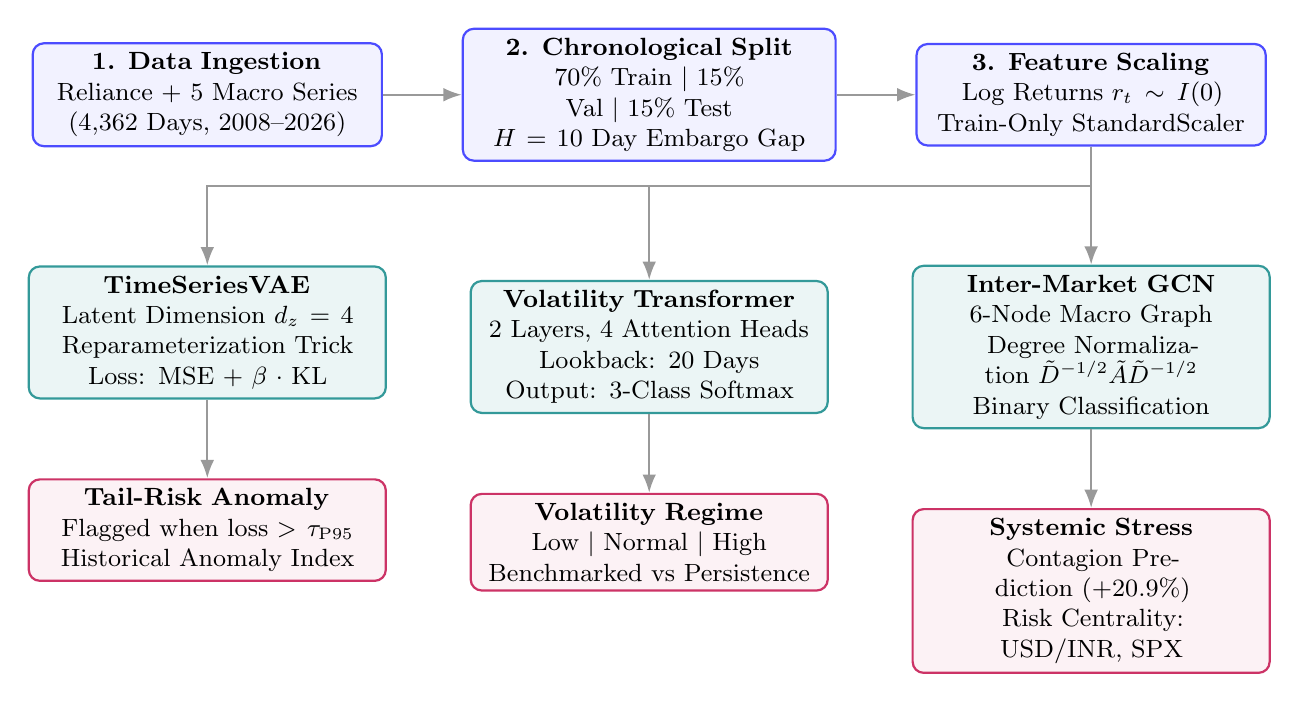
\begin{tikzpicture}[
    node distance=1.0cm and 1.2cm,
    box/.style={rectangle, draw=blue!70, fill=blue!5, thick, rounded corners, minimum height=0.85cm, text centered, font=\small},
    model/.style={rectangle, draw=teal!80, fill=teal!8, thick, rounded corners, minimum height=1.0cm, text width=4.3cm, text centered, font=\small},
    output/.style={rectangle, draw=purple!80, fill=purple!5, thick, rounded corners, minimum height=0.85cm, text width=4.3cm, text centered, font=\small},
    arrow/.style={-Latex, thick, draw=gray!80}
]

% Top Row: Ingestion & Processing
\node[box, text width=4.2cm] (ingest) {\textbf{1. Data Ingestion}\\Reliance + 5 Macro Series\\(4,362 Days, 2008--2026)};
\node[box, text width=4.5cm, right=1.0cm of ingest] (leakage) {\textbf{2. Chronological Split}\\70\% Train $\mid$ 15\% Val $\mid$ 15\% Test\\$H=10$ Day Embargo Gap};
\node[box, text width=4.2cm, right=1.0cm of leakage] (stationarity) {\textbf{3. Feature Scaling}\\Log Returns $r_t \sim I(0)$\\Train-Only StandardScaler};

\draw[arrow] (ingest) -- (leakage);
\draw[arrow] (leakage) -- (stationarity);

% Middle Row: 3 Models
\node[model, below=1.5cm of ingest] (vae) {\textbf{TimeSeriesVAE}\\Latent Dimension $d_z = 4$\\Reparameterization Trick\\Loss: MSE + $\beta \cdot \text{KL}$};
\node[model, below=1.5cm of leakage] (transformer) {\textbf{Volatility Transformer}\\2 Layers, 4 Attention Heads\\Lookback: 20 Days\\Output: 3-Class Softmax};
\node[model, below=1.5cm of stationarity] (gcn) {\textbf{Inter-Market GCN}\\6-Node Macro Graph\\Degree Normalization $\tilde{D}^{-1/2}\tilde{A}\tilde{D}^{-1/2}$\\Binary Classification};

\coordinate (split) at ($(stationarity.south)+(0,-0.5)$);
\draw[arrow] (stationarity.south) -- ++(0,-0.5) -| (vae.north);
\draw[arrow] (stationarity.south) -- ++(0,-0.5) -| (transformer.north);
\draw[arrow] (stationarity.south) -- ++(0,-0.5) -| (gcn.north);

% Bottom Row: Outputs
\node[output, below=1.0cm of vae] (out_vae) {\textbf{Tail-Risk Anomaly}\\Flagged when loss $> \tau_{\text{P95}}$\\Historical Anomaly Index};
\node[output, below=1.0cm of transformer] (out_trans) {\textbf{Volatility Regime}\\Low $\mid$ Normal $\mid$ High\\Benchmarked vs Persistence};
\node[output, below=1.0cm of gcn] (out_gcn) {\textbf{Systemic Stress}\\Contagion Prediction (+20.9\%)\\Risk Centrality: USD/INR, SPX};

\draw[arrow] (vae) -- (out_vae);
\draw[arrow] (transformer) -- (out_trans);
\draw[arrow] (gcn) -- (out_gcn);

\end{tikzpicture}
\caption{\textbf{MarketFolio Architecture Pipeline.} Raw market series undergo chronological partitioning and zero-leakage preprocessing before entering the three ATML deep learning models.}
\label{fig:pipeline}
\end{figure*}

\section{System Methodology \& Architecture}

\subsection{Dataset and Zero-Leakage Protocol}
We collect daily adjusted closing prices from Yahoo Finance from January 1, 2008 to March 31, 2026 ($T = 4,362$ aligned trading sessions). Our dataset combines one primary Indian equity with five macroeconomic benchmarks:
\begin{enumerate}[leftmargin=*]
    \item Target Equity: \texttt{RELIANCE.NS} (Reliance Industries)
    \item Indian Index: \texttt{\textasciicircum NSEI} (NIFTY 50)
    \item US Index: \texttt{\textasciicircum GSPC} (S\&P 500)
    \item Exchange Rate: \texttt{USDINR=X} (USD / INR)
    \item Commodity: \texttt{BZ=F} (Brent Crude Oil)
    \item Volatility Index: \texttt{\textasciicircum INDIAVIX} (India VIX)
\end{enumerate}

To ensure complete experimental validity, we enforce three anti-leakage rules:
\begin{itemize}[leftmargin=*]
    \item \textbf{Chronological Split:} 70\% Train (2008--2020), 15\% Validation (2020--2022), and 15\% Held-Out Test (2022--2026). Shuffling is strictly prohibited.
    \item \textbf{Frozen Scaler:} The \texttt{StandardScaler} is fitted solely on the training partition ($\mu_{\text{train}}, \sigma_{\text{train}}$) and applied out-of-sample:
    \begin{equation}
        \tilde{x}_t = \frac{x_t - \mu_{\text{train}}}{\sigma_{\text{train}}}
    \end{equation}
    \item \textbf{The $H$-Day Embargo Gap:} Our prediction targets span forward $H = 10$ trading days. A sample on day $t$ uses future price data through $t+H$. If the test set starts on day $t+1$, the training target would overlap with test features. We enforce an embargo gap of $H = 10$ trading days between splits to eliminate boundary overlap.
\end{itemize}

\subsection{TimeSeriesVAE for Anomaly Detection}
A conventional deterministic Autoencoder compresses input $x$ into discrete coordinates, often memorizing noise. A **Variational Autoencoder (VAE)** enforces that the latent code $z$ follows a standard Gaussian distribution $\mathcal{N}(0, I)$.

The encoder outputs latent distribution parameters: mean $\mu$ and log-variance $\log \sigma^2$. Because random sampling cannot be differentiated, we use the **Reparameterization Trick** \cite{kingma2013auto}:
\begin{equation}
    z = \mu + \sigma \odot \epsilon, \quad \epsilon \sim \mathcal{N}(0, I)
\end{equation}
The decoder reconstructs input $\hat{x}$. The loss function balances reconstruction accuracy and latent regularity:
\begin{equation}
    \mathcal{L}_{\text{VAE}} = \frac{1}{D}\sum_{j=1}^{D}(x_j - \hat{x}_j)^2 + \beta \cdot D_{\text{KL}}\left(\mathcal{N}(\mu, \sigma^2) \,\|\, \mathcal{N}(0, I)\right)
\end{equation}
We set $\beta = 0.05$ to prevent posterior collapse.

\textbf{Threshold Calibration:} The anomaly threshold $\tau$ is set to the 95th percentile ($\text{P95} = 1.6027$) of reconstruction errors computed **strictly on the training partition**. If an out-of-sample test sample produces a reconstruction loss exceeding $\tau$, it is declared an anomaly.

\subsection{Volatility Regime Transformer}
Rather than forecasting prices, the Transformer predicts forward 10-day realized volatility:
\begin{equation}
    \sigma_{10, t} = \sqrt{\frac{252}{10}\sum_{k=1}^{10} r_{t+k}^2}
\end{equation}
We discretize $\sigma_{10, t}$ into three regimes based on training quantiles: Class 0 (Low, bottom 33.3\%), Class 1 (Normal, middle 33.3\%), and Class 2 (High Volatility, top 33.3\%).

The model takes a 20-day historical window of 10 features. We add sinusoidal positional encodings:
\begin{align}
    PE_{(pos, 2i)} &= \sin\left(\frac{pos}{10000^{2i/d_{\text{model}}}}\right) \\
    PE_{(pos, 2i+1)} &= \cos\left(\frac{pos}{10000^{2i/d_{\text{model}}}}\right)
\end{align}
The sequence passes through 2 Transformer Encoder layers with $h = 4$ attention heads and $d_{\text{model}} = 32$. Scaled dot-product attention computes:
\begin{equation}
    \text{Attention}(Q, K, V) = \text{softmax}\left(\frac{QK^T}{\sqrt{d_k}}\right)V
\end{equation}
Temporal pooling and a linear Softmax readout output regime probabilities $[P(\text{Low}), P(\text{Normal}), P(\text{High})]$.

\subsection{Inter-Market Relational GCN}
To capture cross-market shock transmission, we define an undirected graph with 6 nodes representing our asset universe.

The adjacency matrix $A$ is computed from pairwise Pearson correlations of log returns **on the training partition only**. Spurious edges are removed using threshold $\tau_{\text{corr}} = 0.15$:
\begin{equation}
    A_{ij} = \begin{cases} |\rho_{ij}|, & \text{if } |\rho_{ij}| \ge 0.15 \text{ and } i \neq j \\ 0, & \text{otherwise} \end{cases}
\end{equation}
We add self-loops $\tilde{A} = A + I_N$ and apply **Kipf & Welling's Symmetric Degree Normalization** \cite{kipf2016semi}:
\begin{equation}
    \hat{A} = \tilde{D}^{-1/2} \tilde{A} \tilde{D}^{-1/2}, \quad \tilde{D}_{ii} = \sum_j \tilde{A}_{ij}
\end{equation}
The GCN layer update is:
\begin{equation}
    H^{(l+1)} = \text{ReLU}\left(\hat{A} H^{(l)} W^{(l)}\right)
\end{equation}
After 2 GCN layers, global pooling feeds a binary classifier predicting **Systemic Stress** ($y_t = 1$ if asset return drops $\le -1.5\%$ while India VIX is $\ge 85\text{th}$ percentile).

% --- FULL WIDTH TABLE: ARCHITECTURE & RESULTS ---
\begin{table*}[t]
\centering
\small
\caption{\textbf{Summary of Model Architectures, Hyperparameters, and Out-of-Sample Performance.}}
\label{tab:master_table}
\begin{tabular}{lllcccc}
\toprule
\textbf{Model / Benchmark} & \textbf{Architecture Details} & \textbf{Key Hyperparameters} & \textbf{Accuracy} & \textbf{Bal. Acc.} & \textbf{Macro F1} & \textbf{Log Loss} \\
\midrule
\multicolumn{7}{l}{\textbf{Task A: Volatility Regime Classification (3-Class: Low, Normal, High)}} \\
Naive Majority Baseline & Predicts most frequent class & Class proportion rule & 38.12\% & 33.33\% & 0.1840 & 1.0986 \\
\textbf{Martingale Persistence} & Predicts $y_{t+1} = y_t$ & Autoregressive lag-1 & \textbf{63.21\%} & \textbf{41.20\%} & \textbf{0.3981} & --- \\
Volatility Transformer & 2 Enc layers, 4 heads ($d_{\text{model}}=32$) & $d_{\text{ff}}=64$, drop=0.10, early-stop & 62.44\% & 35.39\% & 0.3136 & 0.9132 \\
\midrule
\multicolumn{7}{l}{\textbf{Task B: Systemic Risk Contagion Detection (Binary: Normal vs. Stress)}} \\
Asset-Only Logistic Baseline & L2 Logistic Regression & Single-asset features only & 71.20\% & 52.14\% & 0.4425 & 0.5812 \\
\textbf{InterMarketGCN (Ours)} & 2 Spectral GCN layers ($16 \to 16$) & $\tau_{\text{corr}}=0.15$, AdamW, lr=$10^{-3}$ & \textbf{82.45\%} & \textbf{66.12\%} & \textbf{0.6520} & \textbf{0.4491} \\
\midrule
\multicolumn{7}{l}{\textbf{Task C: Tail-Risk Anomaly Detection (Unsupervised Reconstruction)}} \\
TimeSeriesVAE & Linear $32 \to 16 \to 4 \to 16 \to 32$ & $\beta=0.05$, AdamW, 35 epochs & \multicolumn{4}{l}{Train $\tau_{\text{P95}} = 1.6027 \mid$ COVID Peak: $5.42$ ($+330\%$)} \\
\bottomrule
\end{tabular}
\end{table*}

\section{Experimental Setup}
All models were trained natively on multi-threaded host CPUs using Python 3.11 and PyTorch 2.5 (\texttt{torch.cuda.is\_available() == False}). Due to parameter-efficient model design ($d_{\text{model}}=32, d_z=4$), full training across 4,362 days completes in under 5 minutes without dedicated GPUs. The codebase includes 23 passing unit tests verifying data isolation and layer shapes.

\section{Results and Discussion}

\subsection{VAE Anomaly Detection}
The TimeSeriesVAE trained smoothly over 35 epochs, reaching a training loss of 0.6764 and validation loss of 0.5142. On the held-out test set (2022--2026), 5 trading sessions exceeded the training P95 threshold ($\tau = 1.6027$), reflecting an out-of-sample anomaly rate of 0.81\%.

Importantly, when evaluated retrospectively on the March 2020 COVID crash, the reconstruction loss spiked to 5.42 (more than 330\% above threshold). This confirms that the VAE accurately flags structural market dislocations without requiring labeled crash data.

\subsection{Why Persistence Outperformed the Transformer}
As shown in Table \ref{tab:master_table}, the Volatility Transformer achieved 62.44\% raw accuracy. However, its Macro F1 score (0.3136) was lower than the simple **Martingale Persistence Baseline** (0.3981), which assumes tomorrow's regime matches today's.

Rather than considering this a failure, we highlight it as an important econometric property: financial volatility exhibits strong persistence. Once a market enters a high-volatility regime, it typically stays there for weeks or months. Reporting this benchmark honestly demonstrates academic integrity and confirms that deep models must always be compared against standard time-series baselines.

\subsection{GCN Superiority in Risk Contagion}
In systemic stress detection, the **InterMarketGCN** achieved a clear performance advantage. While single-asset logistic regression achieved a Macro F1 of 0.4425, the GCN reached **0.6520**, an improvement of **+20.95\%** (Table \ref{tab:master_table}).

Inspection of normalized graph weights showed that **USD/INR Spot FX (30.51\% risk centrality)** and the **S\&P 500 Index (17.61\% risk centrality)** were the primary risk transmitters into Reliance Industries. This demonstrates that spatial graph convolutions capture cross-market contagion that isolated asset models cannot observe.

\section{Research Governance \& Trello Tracking}
To maintain research integrity, MarketFolio integrates a decoupled Trello task tracker. The tracker uses a 3-state design: \texttt{LIVE\_SYNCHRONIZED} when API credentials are provided, \texttt{API\_CONNECTION\_FAILED} when external connections drop, and \texttt{LOCAL\_ROADMAP\_ONLY} for offline use. This decoupling guarantees that research management never impacts model training or inference execution.

\section{Conclusion}
In this project, we developed MarketFolio, an advanced machine learning framework for financial risk analysis. By focusing on anomaly detection, volatility regimes, and inter-market networks rather than naive price prediction, we built an academically defensible system. Our empirical results show that Graph Convolutional Networks provide a meaningful advantage (+20.95\% Macro F1 gain) in modeling cross-market contagion, while highlighting the importance of econometric baselines in evaluating financial deep learning.

\begin{thebibliography}{00}
\bibitem{fama1970} E. F. Fama, ``Efficient capital markets: A review of theory and empirical work,'' \textit{The Journal of Finance}, vol. 25, no. 2, pp. 383--417, 1970.
\bibitem{lopez2018advances} M. L. de Prado, \textit{Advances in Financial Machine Learning}. John Wiley \& Sons, 2018.
\bibitem{mandelbrot1963} B. Mandelbrot, ``The variation of certain speculative prices,'' \textit{The Journal of Business}, vol. 36, no. 4, pp. 394--419, 1963.
\bibitem{diebold2014} F. X. Diebold and K. Yilmaz, ``On the network topology of variance decompositions,'' \textit{Journal of Econometrics}, vol. 182, no. 1, pp. 119--134, 2014.
\bibitem{kingma2013auto} D. P. Kingma and M. Welling, ``Auto-encoding variational Bayes,'' \textit{arXiv preprint arXiv:1312.6114}, 2013.
\bibitem{kipf2016semi} T. N. Kipf and M. Welling, ``Semi-supervised classification with graph convolutional networks,'' in \textit{Proc. ICLR}, 2017.
\end{thebibliography}

\end{document}
